\section{Controller in frequency domain}

% Framework
\subsection{Framework}
For this part of the work, it has decided to simplify our system and use 2 states instead of 4. The position and speed of the damper are therefore hidden in the force of the actuator, which is still the controllable input of the system.
\begin{figure}[H]
    \centering
    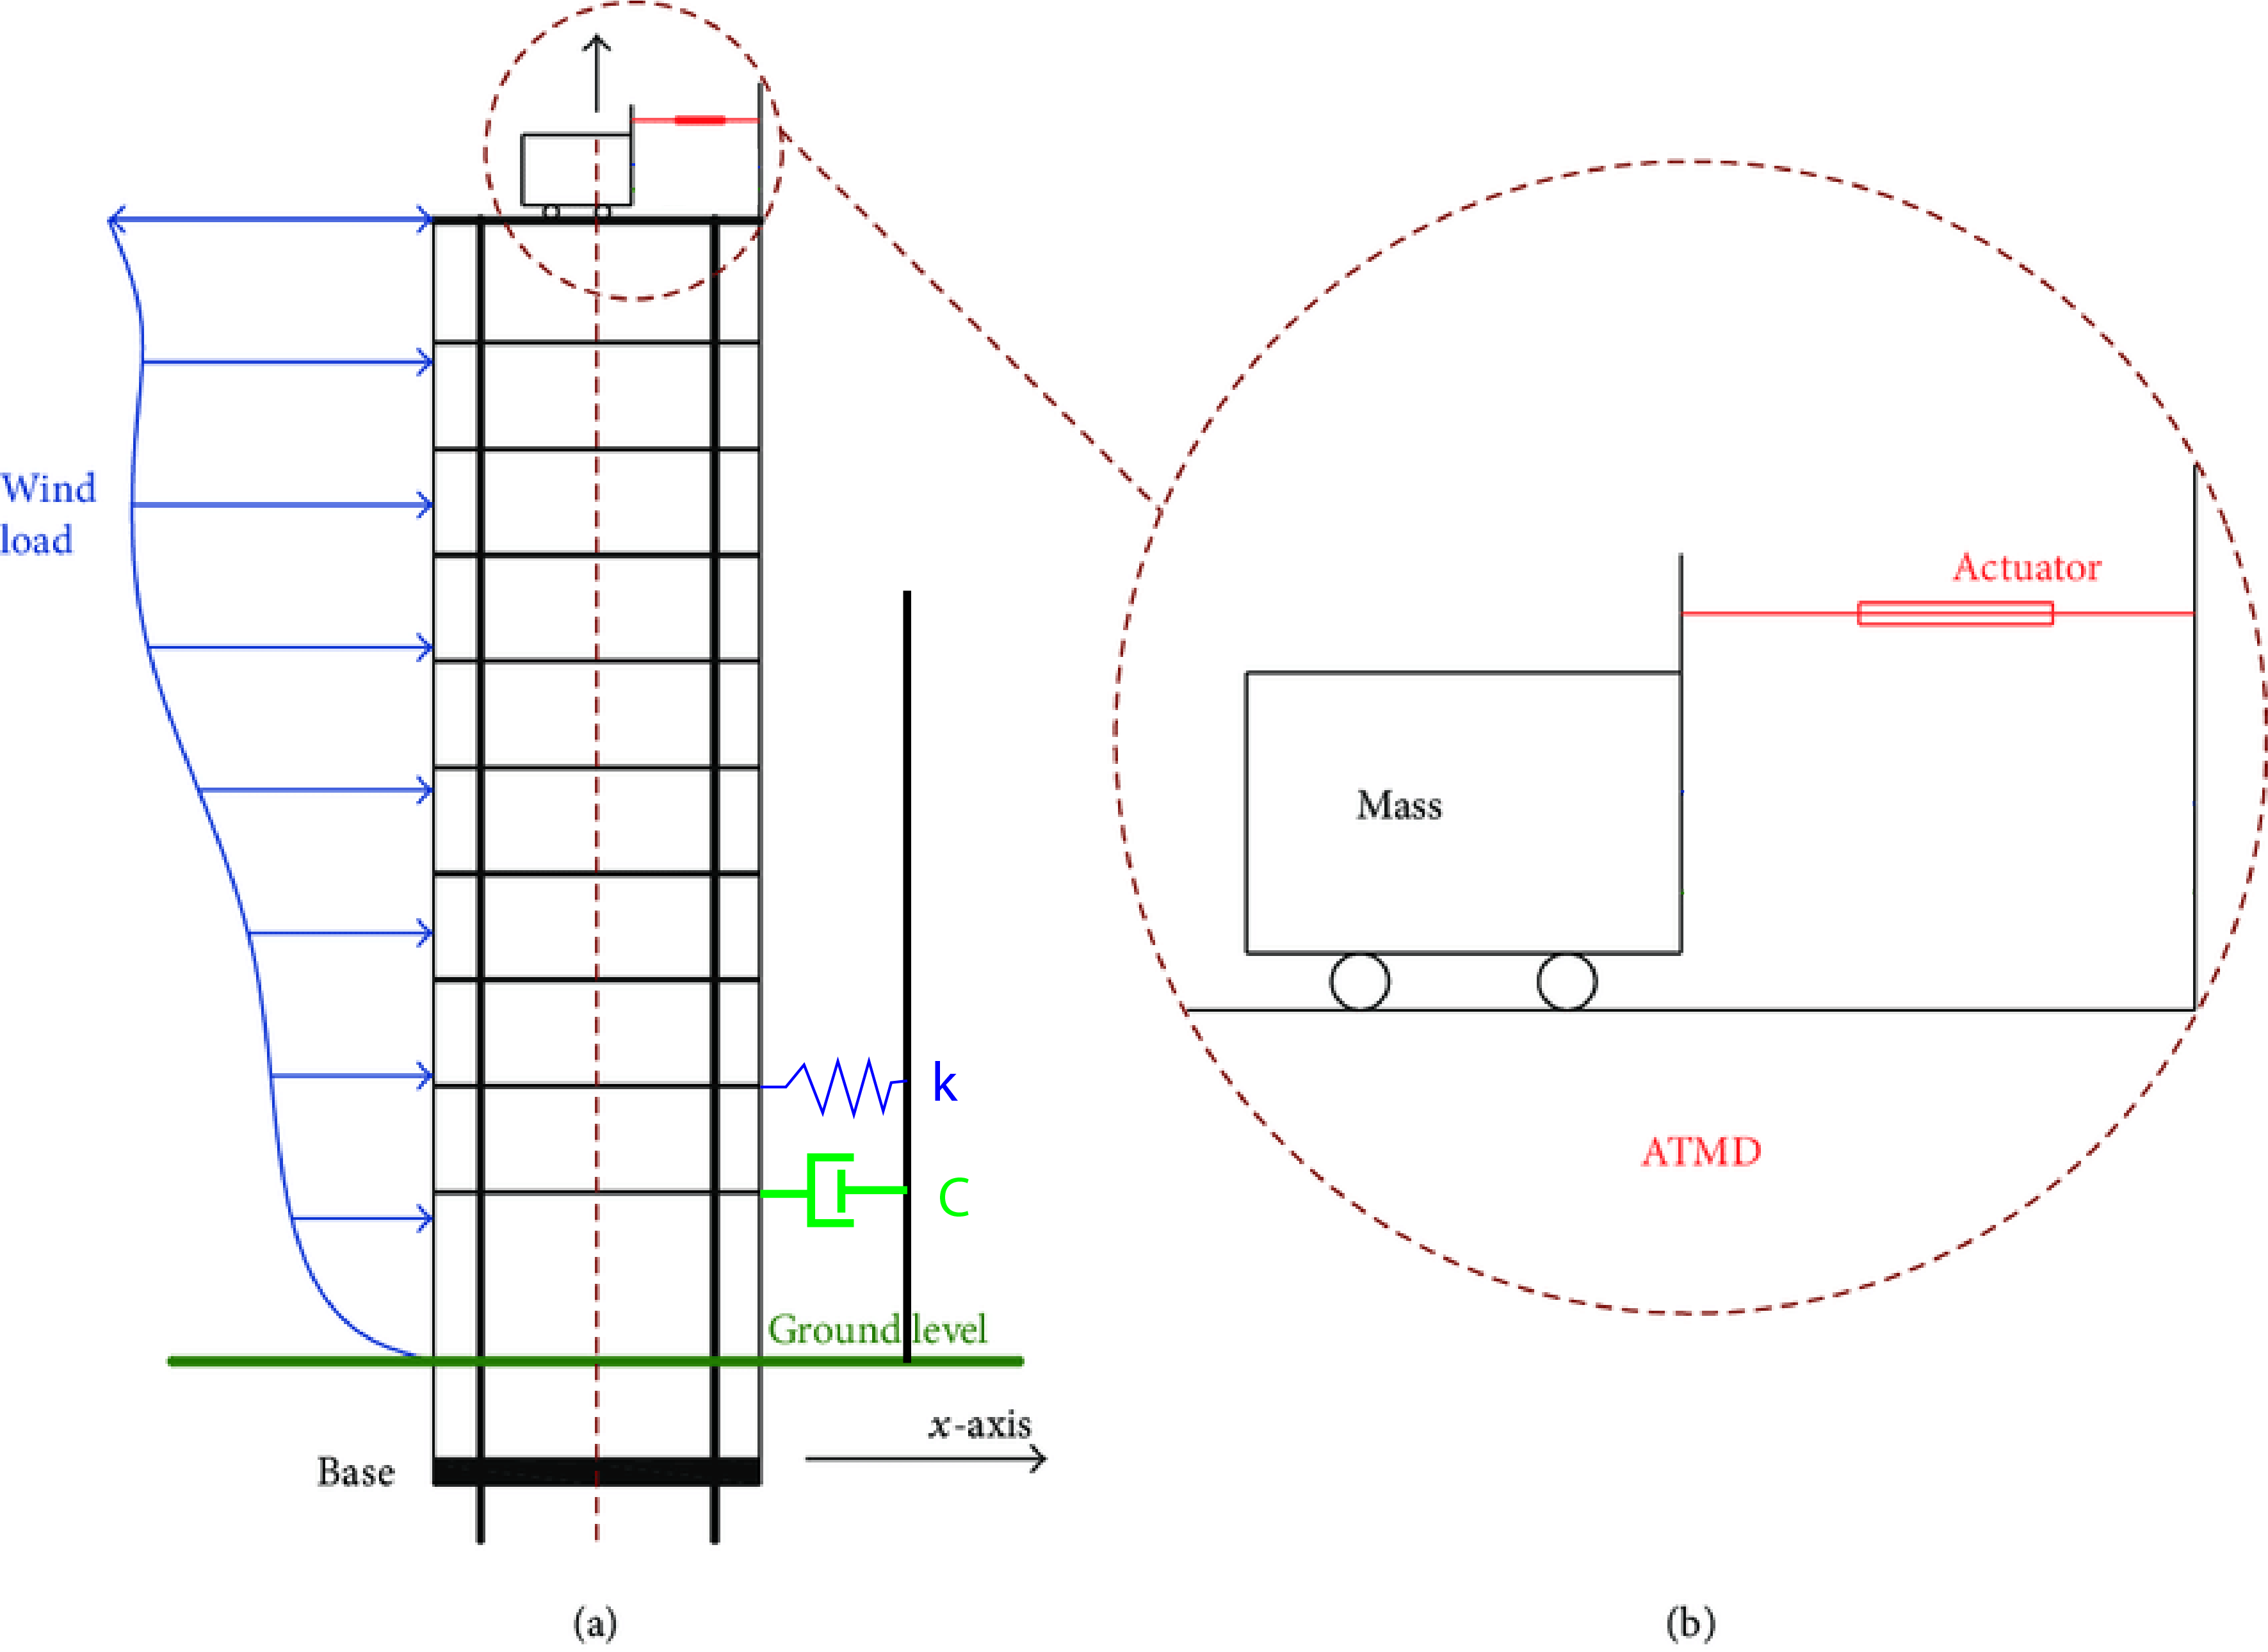
\includegraphics[width=0.7\textwidth]{resources/png/4_simplified-system.png}
    \caption{Simplified system of an active mass damper}
    \label{fig:simplified-system}
\end{figure}
The law that governs that system is the following : 
$$
m_{tot}\ddot{x} + c\dot{x} + kx = F_{wind} + F_{damper}
$$
where
\begin{itemize}
    \item $F_{damper} = m_{damper}a_{damper}$
    \item $m_{tot} = m_{building} + m_{damper}$
    \item $x$ is the position of the building relative to its rest position ($x = 0$)
\end{itemize}
Let's now define the input, output and states : 
\begin{itemize}
    \item $u_1 = F_{wind}$
    \item $u_2 = F_{damper}$
    \item $x_1 = x$
    \item $x_2 = \dot{x}$
    \item $y = x_1$ 
\end{itemize}
By doing so, the ABCD matrices are the following :
$$
A = \begin{pmatrix}
    0 & 1\\
    \dfrac{-k}{m_{tot}} & \dfrac{-c}{m_{tot}}\\
\end{pmatrix}
\quad
B = \begin{pmatrix}
    0 & 0\\
    \dfrac{1}{m_{tot}} & \dfrac{1}{m_{tot}}\\
\end{pmatrix}
$$
$$
C = \begin{pmatrix}
    1 & 0\\
\end{pmatrix}
\quad
D = \begin{pmatrix}
    0 & 0\\
\end{pmatrix}
$$

\subsubsection{Constraints and simulation specifications}
We have the following constraints : 
\begin{itemize}
    \item Acceleration of the mass damper below \num{1.6}$g$, to be consistent with the time domain.
    \item Lateral movement of the top of the building not above \SI{1}{\meter}.
\end{itemize}
The two scenarios we look at are the following : a turbulent wind of maximum \SI{810}{\kilo\newton}, that is represented as a sine function and a constant wind of the same intensity (the random wind has been studied and is referenced but is not plotted for this section).\par
Here are the values of the different parameters that have been chosen, as previously : 
\begin{table}[H]
    \centering
    \begin{tabular}{|l|c|c|}
        \hline
        {\bf Mass} & $m_{building} = \SI{1e7}{\kilogram}$ & $m_{damper} = \SI{3e4}{\kilogram}$\\ \hline
        {\bf Spring} & \multicolumn{2}{c|}{$k\approx\SI{4e8}{\newton\per\meter}$}\\ \hline
        {\bf Damper} & \multicolumn{2}{c|}{$c\approx\SI{1.3e6}{\newton\second\per\meter}$}\\ \hline
        {\bf Wind} & \multicolumn{2}{c|}{$F_{max} = \SI{810}{\kilo\newton}$}\\ \hline
    \end{tabular}
    \caption{Numerical values of the system}
    \label{tab:numerical-values}
\end{table}

\subsubsection{Choice of cross-over frequency}
The frequency of the building is of about \SI{1}{\hertz}, as advised by Pr. Denoël, and the frequency of the sinusoidal wind studied is also of \SI{1}{\hertz}. So the cross-over frequency was initially set at \SI{5}{\hertz}.\par
All frequencies above that, probably coming from noise and unwanted phenomena, will be attenuated, while the amplitudes of the frequencies below that, which correspond to the internals of the system, will be amplified.\par
In the end, after some simulations, we have decided to put the crossover frequency at \SI{20}{\radian\per\second} as we have found out that a smaller crossover frequency induces a slightly slower response in our system. Although not noticeable in the sinusoidal force scenario, it can be seen when the disturbance is a constant or a random function.

% Transfer function of the open-loop system
\subsection{Transfer function of the open-loop system}
\subsubsection{Computation}
For the computation of the transfer function of our system, we used the Matlab function \texttt{tf(sys)} then selecting the answer corresponding to our controllable input. In our case,
$$
P(s) = \dfrac{9.97e-8}{s^2 + 0.1257s + 39.48}
$$
Had we wanted to compute it by hand, we would have translated our ABCD system to its frequency form (derivative becomes a multiplication by $s$), then we would have found that
$$
H(s)=\frac{Y(s)}{U(s)}=C(s I-A)^{-1} B+D
$$
By selecting only the columns of B and D corresponding to the controllable input, we would have found the same expression as the one above.

\subsubsection{Plots}
The Bode plots of the open-loop system are given at figure \ref{fig:bode-ol}.
\begin{figure}[H]
    \centering
    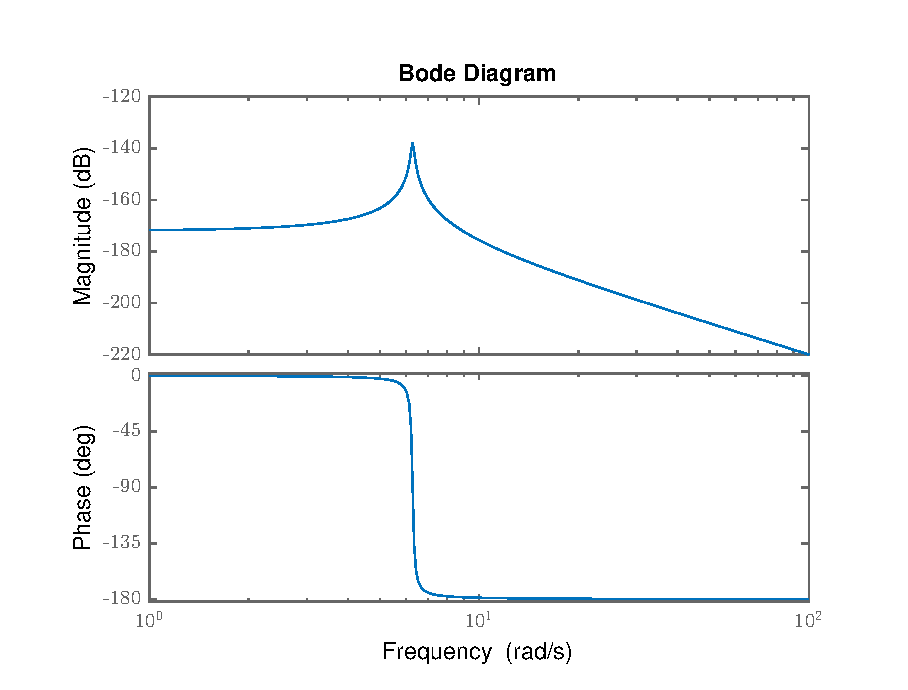
\includegraphics[scale=0.8]{resources/eps/4-Val/bode-ol.eps}
    \caption{Bode plots for 2D system}
    \label{fig:bode-ol}
\end{figure}
These graphs have the typical shape of the second order systems. If we confront our transfer function with the typical transfer function of such a system ($H(s)=\frac{1}{s^{2}+2 \zeta \omega_{n} s+\omega_{n}^{2}}$), we find that $\omega_n\approx6.28$ and $\zeta \approx 0.01$.\par
We thus have two complex poles, oscillations and overshoots. The peak is quite high, as $\zeta \ll 1$, and the transition from \SI{0}{\degree} to \SI{-180}{\degree} (at $\omega_n$, the natural frequency of our system) is quite sharp for the same reasons.

% Loop shaping
\subsection{Loop shaping}
\subsubsection{Lag compensator}
Firstly, we have decided to use a lag compensator in order to increase the gain for low frequencies (remove the flat area at low frequencies) and thus have a better response. We have used a lag compensator of the following shape :
$$
Glag(s) = \dfrac{s + a}{s}
$$
The bode diagram of that transfer function is given at figure \ref{fig:glag}.
\begin{figure}[H]
    \centering
    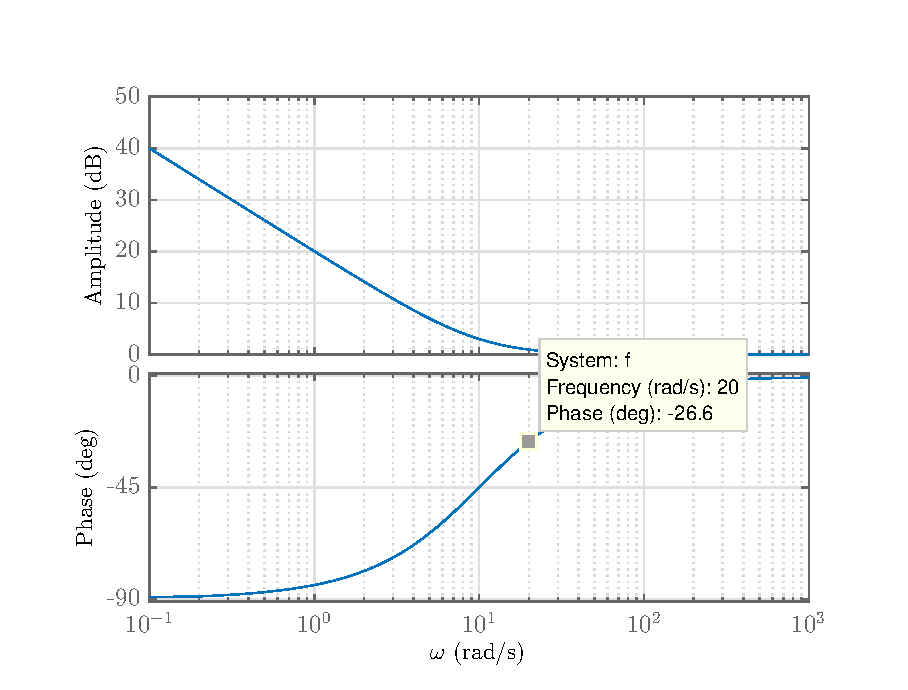
\includegraphics[scale = 0.8]{resources/eps/4-Val/glag.eps}
    \caption{Bode diagrams of the lag compensator}
    \label{fig:glag}
\end{figure}
We have decided to use a $a$ of $10$ to attenuate the natural frequency spike in the initial Bode amplitude diagram without interfering too much with the phase diagram ($a$ is used to move the point at which the amplitude of the Bode diagram becomes \SI{0}{\deci\bel}).\par
As can be seen, this element induces a phase of about \SI{-26}{\degree} at the crossover frequency, but it is not a problem as we have succeeded in tuning our lead compensator to be resistant to the delays we will have in our system. It can be noted that, for a sinusoidal wind, the use of such a component is not necessary. However, when we conducted tests with a constant wind (equivalent to a step), we have found out that using a lag compensator induces no static error while not using one induces a stabilization at a position different from the reference.\par
However, the acceleration of the damper becomes twice as large as those with no lag compensator. We have decided to keep it to comply with the theoretical shape of the desired Bode diagram but, in practice, if the acceleration is too intense with such a component, we could easily remove it without bringing instabilities in the response of the building.

\subsubsection{Lead compensator}
Let's now add a lead compensator to obtain the desired phase margin. Delays are discussed after, but we want to be able to respond at least to \SI{0.02}{\second} delays, which correspond to the \SI{50}{\hertz} of the actuator's piston \cite{Hassan_2016}.\par
We have finally decided to use a phase margin of \SI{80}{\degree} for the following computations, although it will translate in practice to a phase margin of \SI{42}{\degree} because of interference with the lag compensator and the low-pass filter. In order to increase the phase margin at the crossover frequency, we have decided to use a lead compensator.\par
Its transfer function is given by : 
$$
G(s) = \dfrac{\frac{s}{w_z} + 1}{\frac{s}{w_p} +1}
$$
For a given crossover frequency $\omega_{co}$ and a phase margin $\phi_m$, we can determine the two $w$ (further apart means a phase and amplitude modifications in $L$ more spread) in the following way : 
$$
\left\{\begin{array}{l}
    {w_{z}=\tan (\alpha) w_{\mathrm{co}}} \\
    {w_{p}=\frac{w_{\mathrm{co}}}{\tan (\alpha)}}
\end{array}\right.
$$
with $\alpha = \frac{\pi}{4} - \frac{\phi_m}{2}$.\par
For the crossover frequency and the desired value of $\phi_m$, we have that that : 
$$
w_z = \num{1.75} \qquad w_p = \num{228.6}
$$
We have chosen that phase margin because, with one below \SI{65}{\degree}, the delays we have determined bring instability to our system, as we have seen in the Nyquist diagrams. Any value above that is fine in that regards and does not impact our output and controllable input in a very determinant way. However, lower phase margins tend to slightly increase the speed of our control system, so we have chosen this phase margin of \og{}\SI{80}{\degree}\fg{}. The Bode plots of this component is given at figure  \ref{fig:glead}.
\begin{figure}[H]
    \centering
    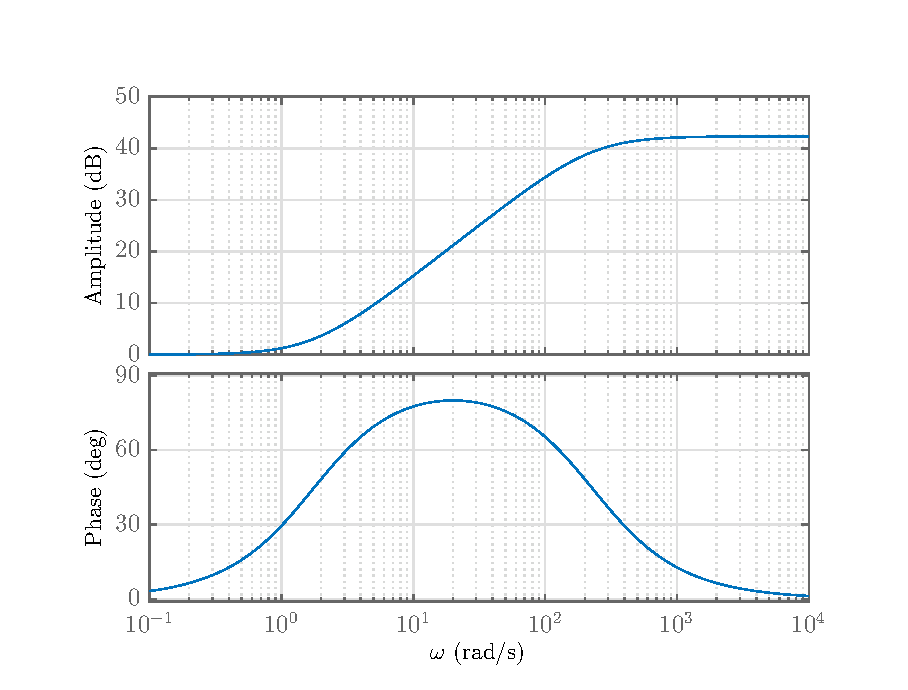
\includegraphics[scale = 0.8]{resources/eps/4-Val/glead.eps}
    \caption{Bode diagrams of the lead compensator}
    \label{fig:glead}
\end{figure}

\subsubsection{Gain}
After that, one needs to add a gain to our system in order to increase the amplitude gains for all frequencies and make it so that the amplitude is at \SI{0}{\deci\bel} at the crossover frequency. That is done by using a constant gain. This does not affect the phase but increases the amplitudes of about \SI{175.5}{\deci\bel}, which positions our Bode plot to where one wanted it to be. 

\subsubsection{Low-Pass Filter}
$$
G(s) = \dfrac{1}{\frac{s}{a}+1}
$$
We have decided to use a low-pass filter in order to attenuate even more the gains for higher frequencies.\par
In the case of a random wind, we have seen that it reduces a bit the spikes in the controllable input, so we have decided to keep it, although its action for other scenarios was not perceived. However, such a filter is designed to attenuate the effect of noise on the system, and in that regards, it works quite well with our system, as we can see in the section dedicated to noise at the end of this report.\par
As can be seen on the Bode diagrams at the figure \ref{fig:lpf}, we induce a loss in phase of about \SI{11}{\degree} by choosing a parameter $a = 5*\omega_{co}$ for the low-pass filter. However, as it has already been said for the lag compensator, the system can still react well to the delays we have identified. If it did not, we could use a bigger $a$, but we would react less nicely to noise.
\begin{figure}[H]
    \centering
    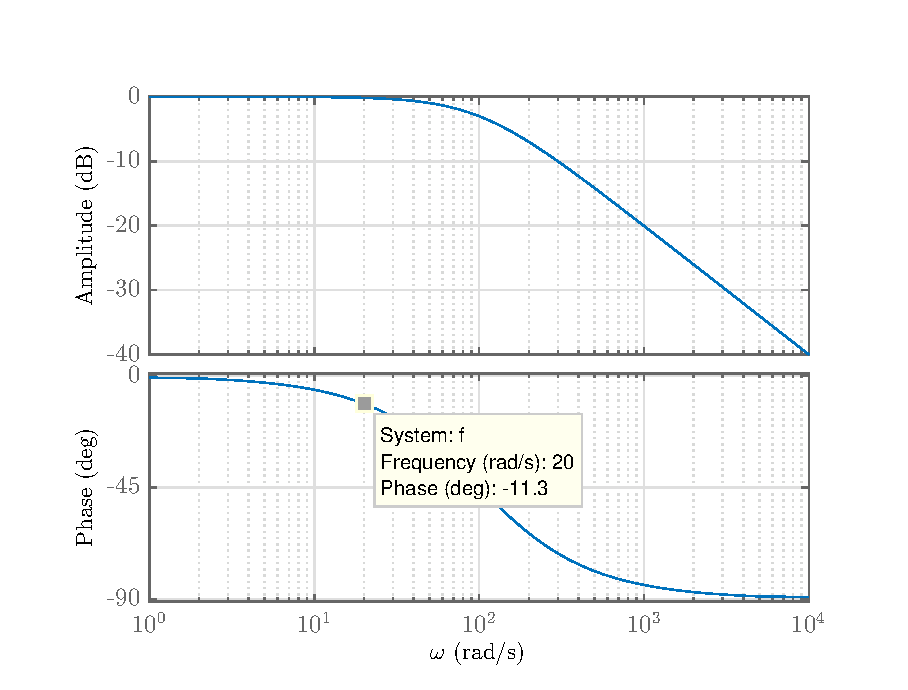
\includegraphics[scale = 0.8]{resources/eps/4-Val/lpf.eps}
    \caption{Bode diagrams of the low-pass filter}
    \label{fig:lpf}
\end{figure}

\subsubsection{Trade-offs}
The Bode and Nyquist plots of the controlled system are given at figures \ref{fig:bode-control} and \ref{fig:nyquist-control}. The different tradeoffs that had to be made are explicited in the different sections concerning the components we have used. We had to make compromises for the phase margin, the rejection of noise and the use of a lag compensator.\par
Concerning the output and the controllable input (Figures \ref{fig:controllable-input} and \ref{fig:output}, \ref{fig:controllable-input2} and \ref{fig:output2}), we can see that the damping is very well obtained, although the force needed for the damper is a bit over what we have used in our constraints (not using a lag compensator brings us below them in the case of a constant wind but not in the case of a sinusoidal one). We have tried numerous changes in parameters to go below these constraints for the sinusoidal wind but have not succeeded.
\begin{figure}[H]
    \centering
    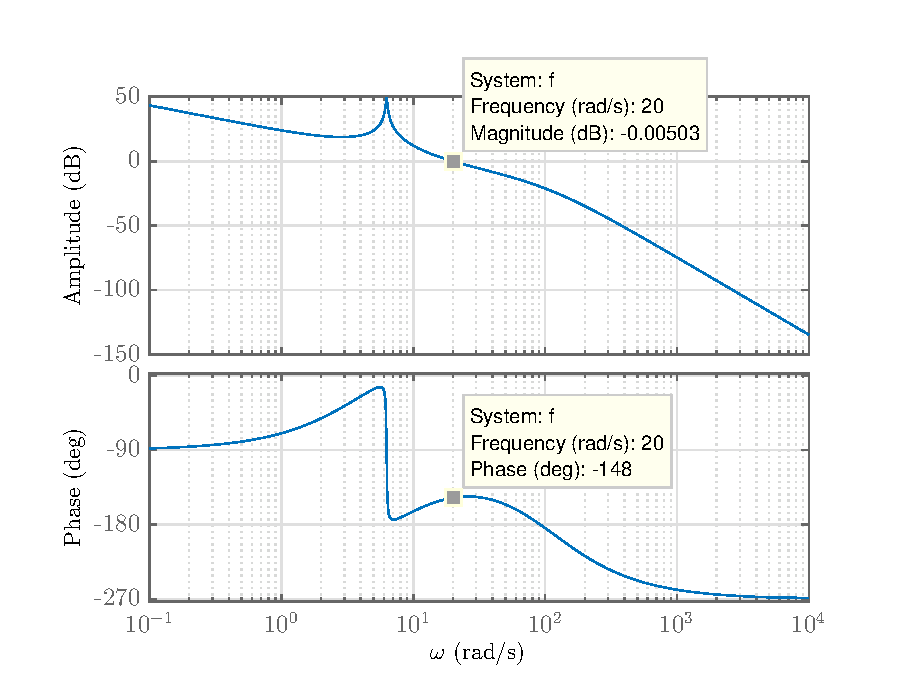
\includegraphics[scale = 0.8]{resources/eps/4-Val/L.eps}
    \caption{Bode plots of the controlled system}
    \label{fig:bode-control}
\end{figure}
\begin{figure}[H]
    \centering
    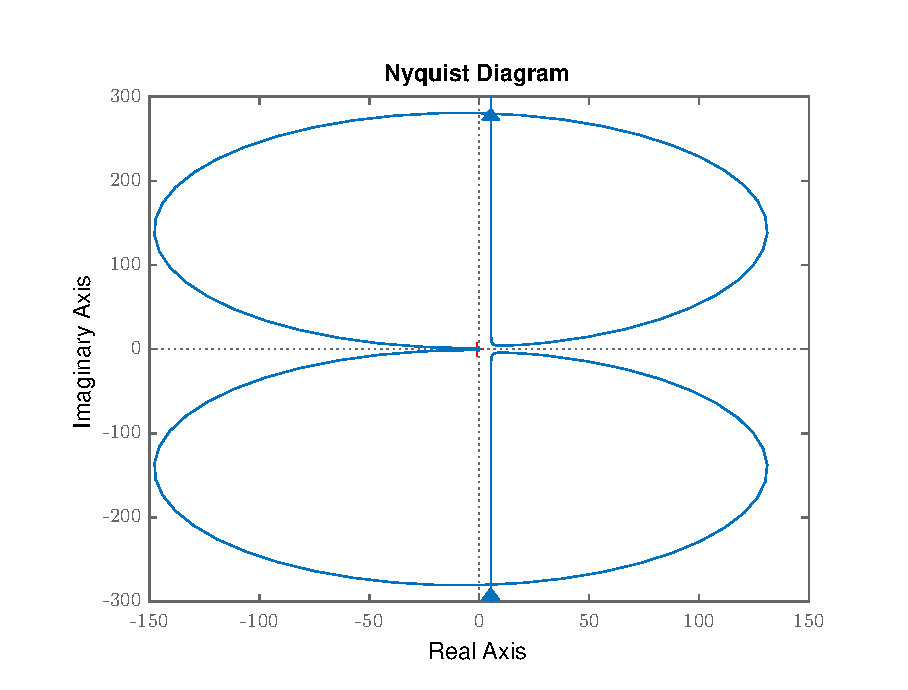
\includegraphics[scale = 0.8]{resources/eps/4-Val/L_nyq.eps}
    \caption{Nyquist plot of the controlled system}
    \label{fig:nyquist-control}
\end{figure}
\begin{figure}[H]
    \centering
    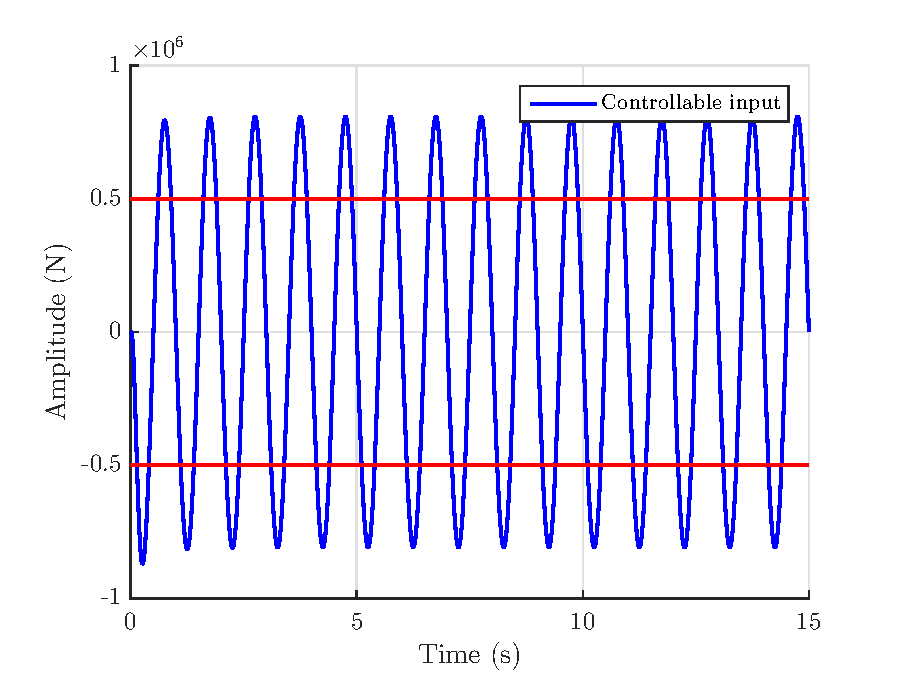
\includegraphics[width=0.8\textwidth]{resources/eps/4-Val/sin_force.eps}
    \caption{Plot of the controllable input of the controlled system subjected to sinusoidal wind}
    \label{fig:controllable-input}
\end{figure}
\begin{figure}[H]
    \centering
    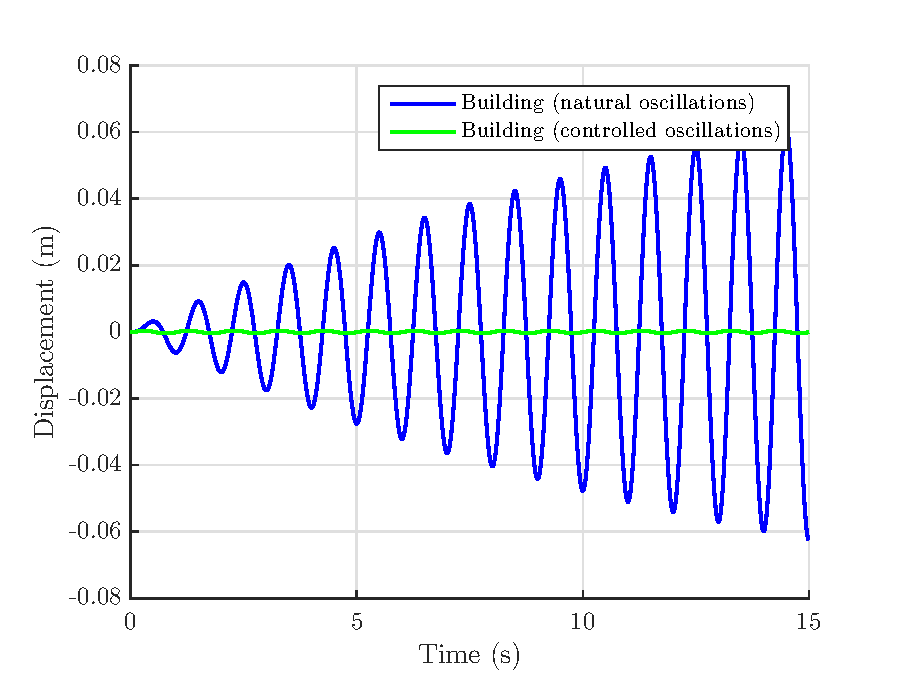
\includegraphics[width=0.8\textwidth]{resources/eps/4-Val/sin_building.eps}
    \caption{Plot of the output of the controlled system subjected to sinusoidal wind}
    \label{fig:output}
\end{figure}
\begin{figure}[H]
    \centering
    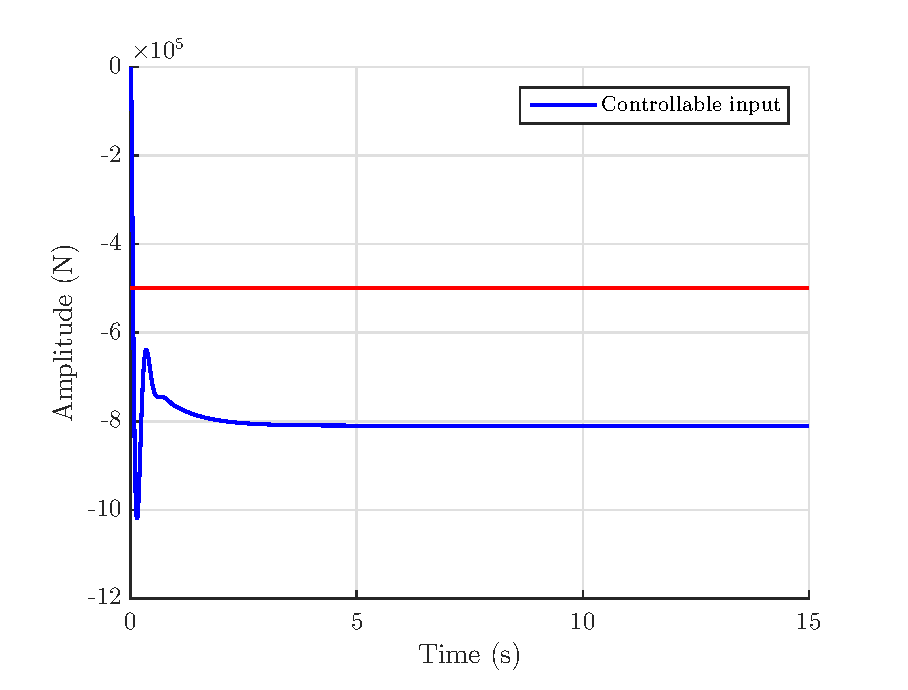
\includegraphics[width=0.8\textwidth]{resources/eps/4-Val/cst_force.eps}
    \caption{Plot of the controllable input of the controlled system subjected to a constant wind}
    \label{fig:controllable-input2}
\end{figure}
\begin{figure}[H]
    \centering
    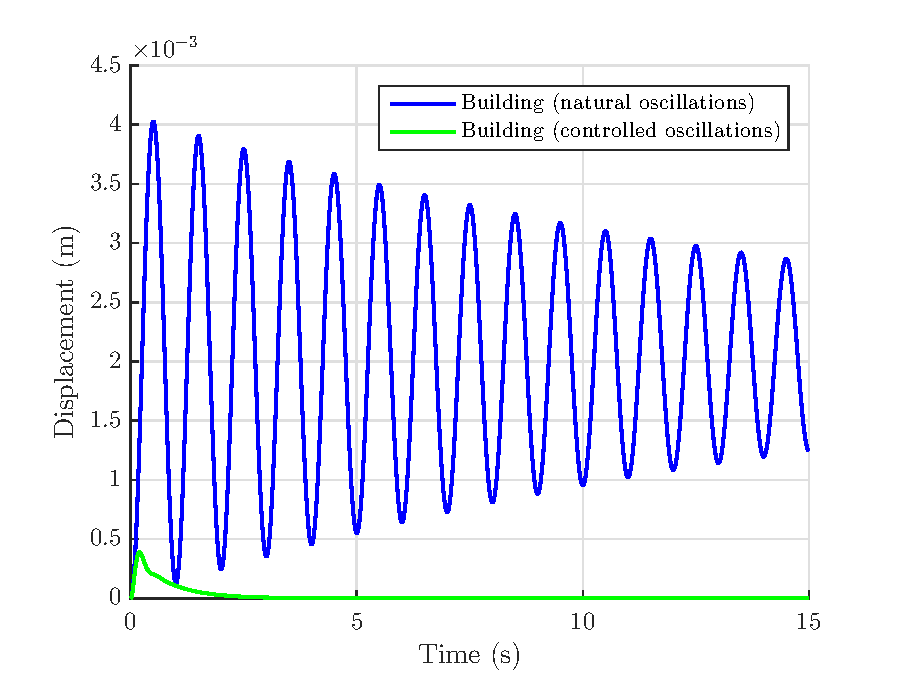
\includegraphics[width=0.8\textwidth]{resources/eps/4-Val/cst_building.eps}
    \caption{Plot of the output of the controlled system subjected to a constant wind}
    \label{fig:output2}
\end{figure}

% Gang of four
\subsection{Gang of four}
\subsubsection{Sensitivity function}
$$
S(s) = \dfrac{1}{1 + PC}
$$
The Bode plots of the sensitivity function are given at figure \ref{fig:sensitivity}. That function tells how the noise acts on the output. We do not want the system to react to the noise, as it is actually the measurement noise that must stay in the output.\par
As noise is a high-frequency phenomenon, we want to have no attenuation of high frequencies in the Bode plot of $S$. As can be seen, it is the case. We have a gain of $0$dB for higher frequencies.\par
In the amplitude graph, we can see a small bump before stabilizing at $0dB$. That is the stability margin, which should remain small. It is not too high in our case, as the maximum sensitivity $M_s = 3.1dB$ and it occurs between $23$ and $24$ rad/s. As the stability margin is equal to the inverse of $M_s$, a high value for $M_s$ would induce a small stability margin and larger amplifications of the disturbances.\newline
\paragraph{Remark}If we wanted a lower gain for lower frequencies (better resistance to disturbance), we would have a greater $M_s$ as, due to Bode's integral formula, the integral of $\log(|S|)$ over $R^+$ is equal to $0$ (waterbed effect). 
\begin{figure}[H]
    \centering
    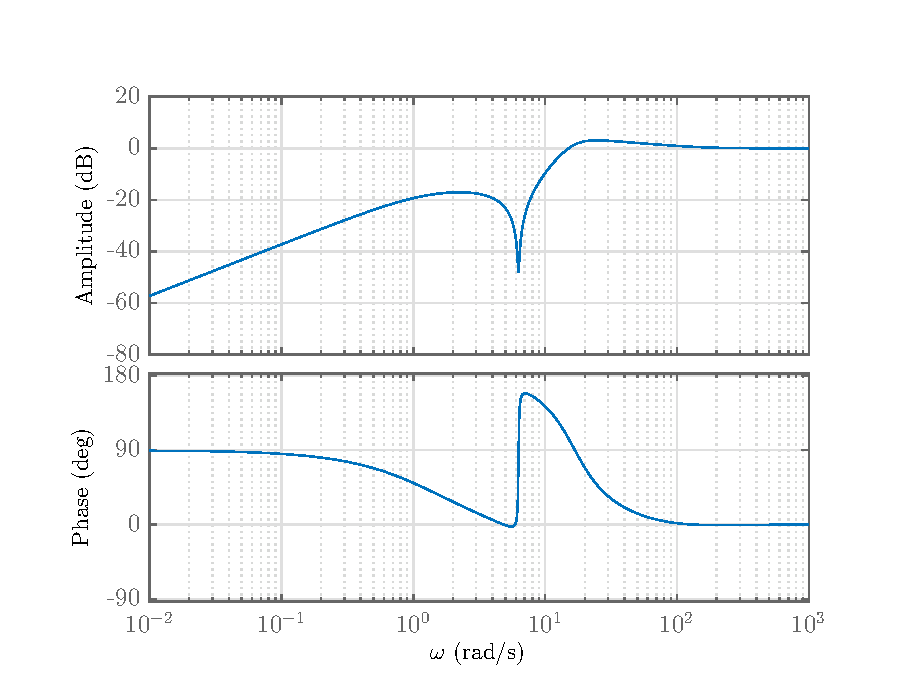
\includegraphics[scale = 0.8]{resources/eps/4-Val/S.eps}
    \caption{Bode plots of the sensitivity function}
    \label{fig:sensitivity}
\end{figure}

\subsubsection{Load sensitivity function}
$$
PS(s) = \dfrac{P}{1 + PC}
$$
This function tells how the disturbances act on the output and the Bode diagrams are given at figure \ref{fig:load}. The system needs to be robust against disturbances. In the present case, these disturbances are low frequency phenomena (frequency of the wind, which we have either chosen constant or a sine function of frequency equal to 1 Hz). We can see that we have a very good reaction concerning the effect of the wind on the output of the system (attenuation of about \SI{-200}{\deci\bel}).
\begin{figure}[H]
    \centering
    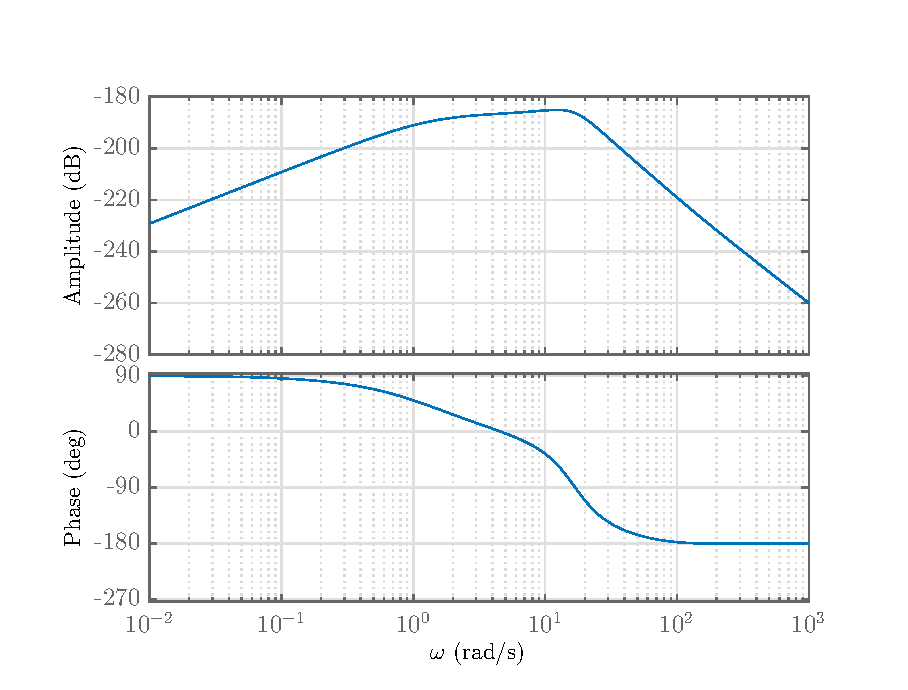
\includegraphics[scale = 0.8]{resources/eps/4-Val/PS.eps}
    \caption{Bode plots of the load sensitivity function}
    \label{fig:load}
\end{figure}

\subsubsection{Complementary sensitivity function}
$$
T(s) = \dfrac{PC}{1 + PC}
$$
This function tells us how the disturbances act on the controllable input and the reference acts on the output and the controllable input, and the Bode diagrams are given at figure \ref{fig:complementary-sensitivity}.\par
The control signal must be reactive to disturbance and the output should be able to track the reference. Amplitudes at low frequency should therefore not be dampened, and one sees that they are not attenuated on the plots. After the maximum complementary sensitivity $M_t$, we have a decreasing slope in amplitude which makes it so that high frequency phenomena (such as noise) are attenuated. (As $S$ + $T$ = 1, we can see that we have a tradeoff between resistance to noise and resistance to disturbance. Better resistance to one induces a worse resistance to the other.)
\begin{figure}[H]
    \centering
    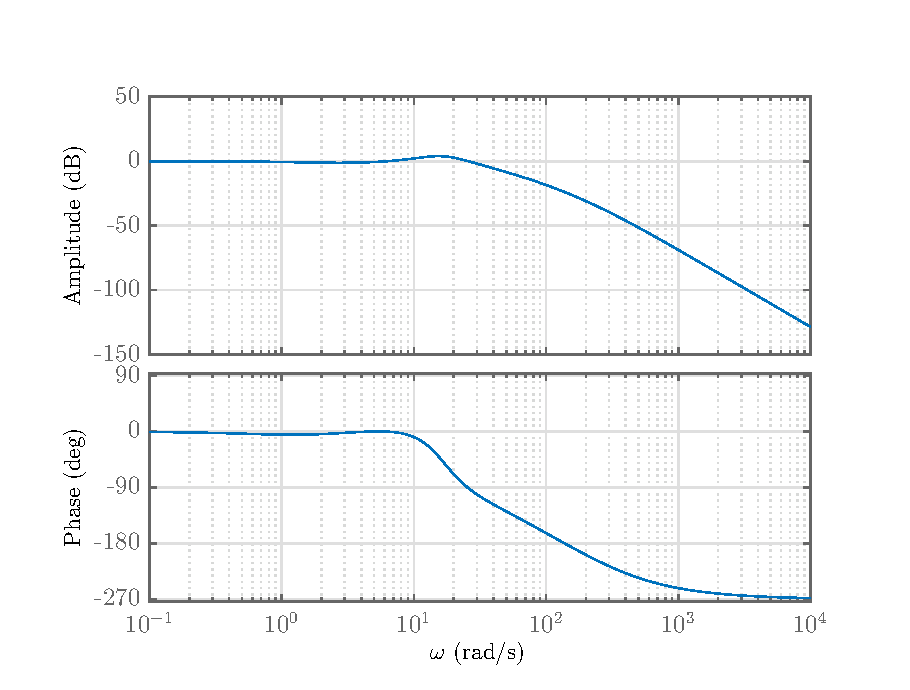
\includegraphics[scale = 0.8]{resources/eps/4-Val/T.eps}
    \caption{Bode plots of the complementary sensitivity function}
    \label{fig:complementary-sensitivity}
\end{figure}

\subsubsection{Noise sensitivity function}
$$
CS(s) = \dfrac{C}{1 + PC}
$$
This function tells us how the noise and the reference act on the controllable input, and the Bode diagrams are given at figure \ref{fig:noise-sensitivity}.\par
That function should be reactive to reference changes, but not to noise, and so have a high magnitude at low frequency and low magnitude at high frequencies. One can see that it is not the case here. Indeed, one has high amplitudes for high frequencies. However, as our reference does not change in our system (we do not plan on dampening the oscillations in a Pisa Tower), it does not really matter.\par
It is also known that temporal domain controllers are better at reacting to reference changes than frequency domain ones.
\begin{figure}[H]
    \centering
    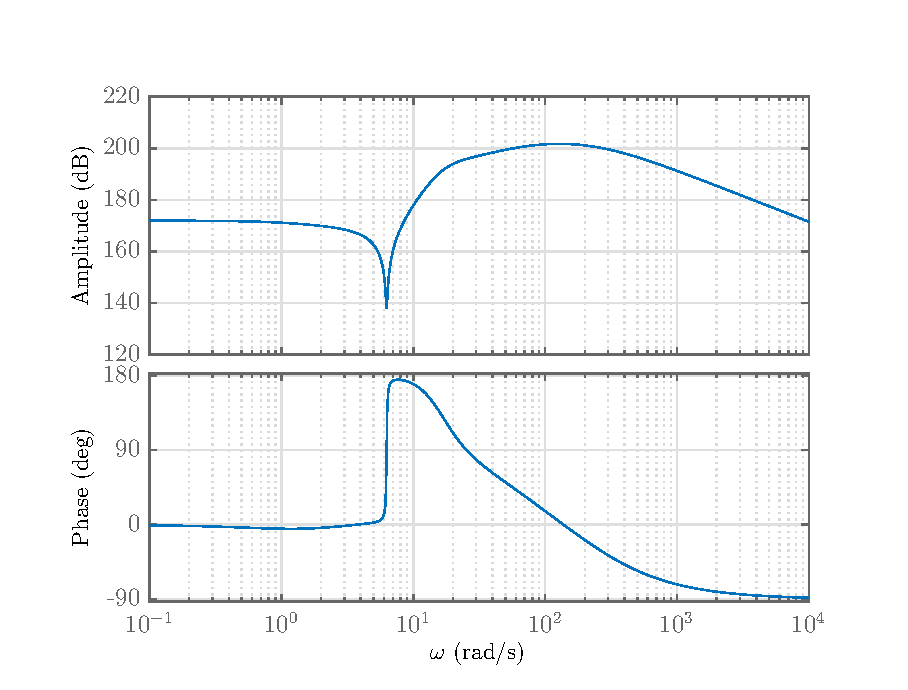
\includegraphics[scale = 0.8]{resources/eps/4-Val/CS.eps}
    \caption{Bode plots of the noise sensitivity function}
    \label{fig:noise-sensitivity}
\end{figure}

% Delays
\subsection{Delays}
The delays in our system are due to the sensor transmitting the information, the microcontroller processing that information and the actuator (piston) actually moving our mass damper. We have chosen that last source of delay as being the biggest one, with a frequency of \SI{50}{\hertz}, which induces delays of \SI{0.02}{\second} (discussed in the lead compensator).\cite{}\par
Some Bode and Nyquist plots showing delays are given at figures \ref{fig:bode-42}, \ref{fig:nyquist-42} and \ref{fig:nyquist-27}. It cannot be seen, but the curve for the delay of $0.02s$ on the Nyquist plot for the lowest phase encompasses the -1 value out of the image.\par
As can be seen, for a phase margin of \SI{42}{\degree}, the delays in our system do not bring instabilities. However, for larger delays, such as the $0.5s$ we have used to simulate Figure \ref{fig:toomuchdelay}, we can clearly see some instabilities in our system. If we wanted to be resistant to such delays, we should increase the phase margin by placing our lag compensator and low-pass filter further away from the crossover frequency.\par
We decided to not include figures comparing the output and the controllable input in the case of delays or not because we ran out of space and we saw almost no difference. The two scenarios reached the same state with only a fraction of a second apart from one another. What happens when the delay is too big, however, is shown in Figure \ref{fig:toomuchdelay}.
\begin{figure}[H]
    \centering
    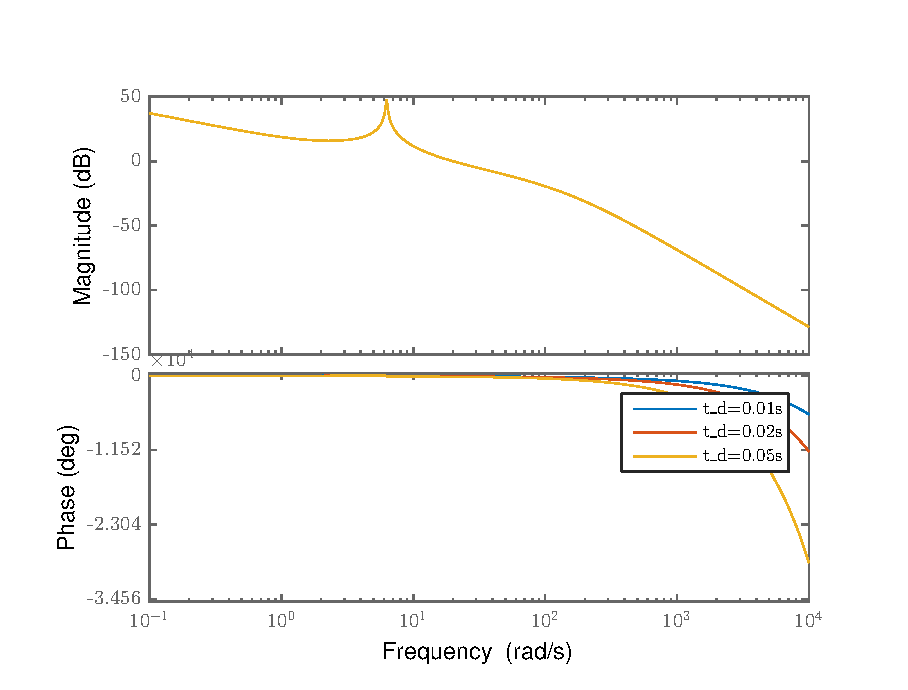
\includegraphics[width=0.8\textwidth]{resources/eps/4-Val/bode_delays.eps}
    \caption{Bode plots for various delays and a phase margin of 42 degrees}
    \label{fig:bode-42}
\end{figure}
\begin{figure}[H]
    \centering
    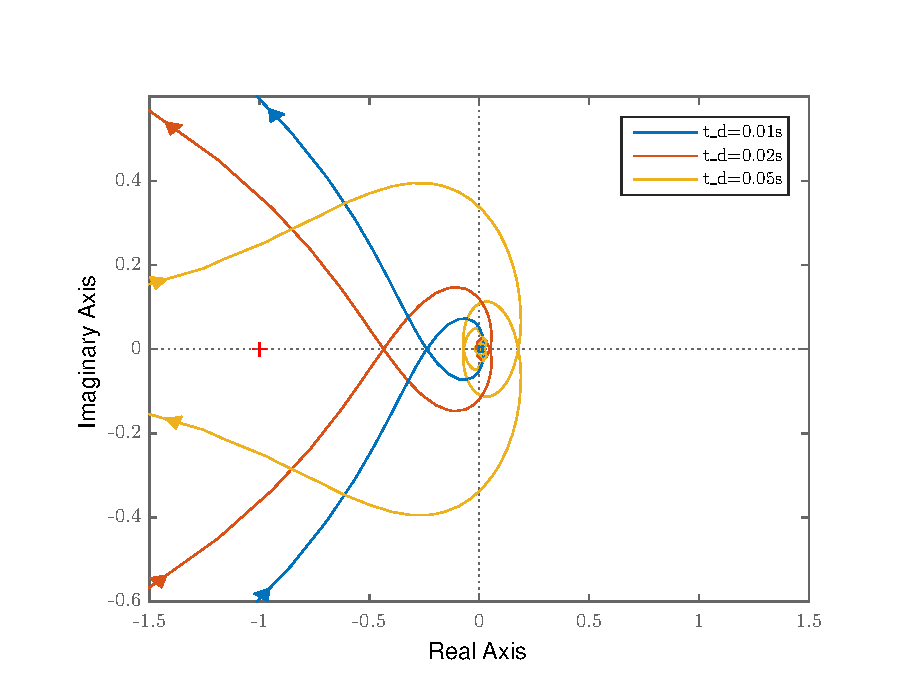
\includegraphics[width=0.8\textwidth]{resources/eps/4-Val/nyq_delay80.eps}
    \caption{Nyquist plots for various delays and a phase margin of 42 degree}
    \label{fig:nyquist-42}
\end{figure}
\begin{figure}[H]
    \centering
    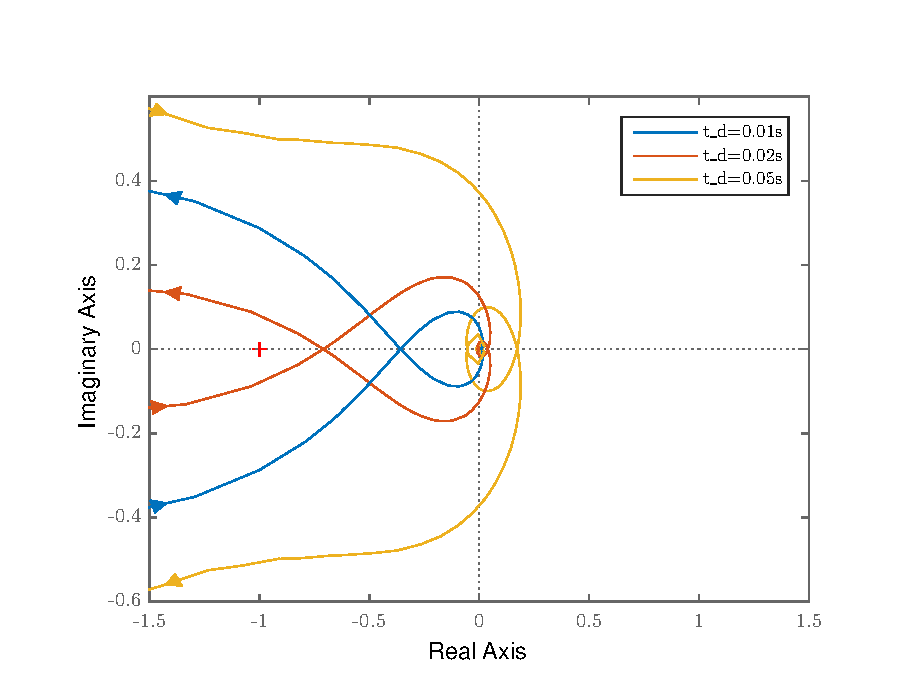
\includegraphics[width=0.8\textwidth]{resources/eps/4-Val/nyq_delay65.eps}
    \caption{Nyquist plots for various delays and a phase margin of 27 degrees}
    \label{fig:nyquist-27}
\end{figure}
\begin{figure}[H]
    \centering
    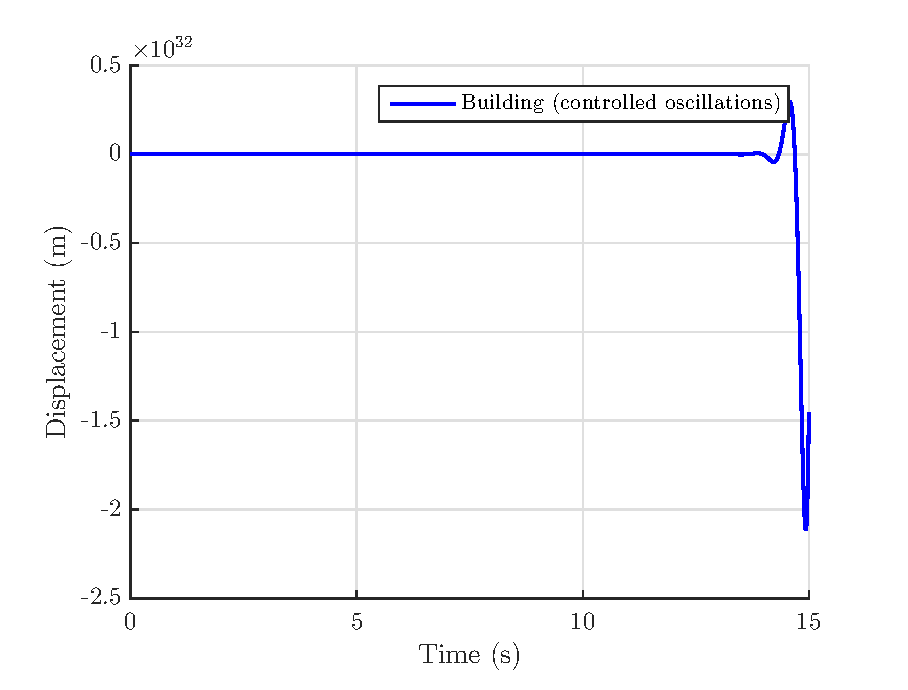
\includegraphics[width=0.8\textwidth]{resources/eps/4-Val/toomuchdelay.eps}
    \caption{Output of our controlled system with a delay of 0.5s}
    \label{fig:toomuchdelay}
\end{figure}

% Noise
\subsection{Noise}
As we can see in Figures \ref{fig:inputnonoise}, \ref{fig:noiselpf} and \ref{fig:noisenolpf}, our system reacts quite well to noise thanks to our low-pass filter. Had we not implemented that filter, we can see that the effect on our controllable input is visible and prone to disturb our control. We did not plot the response of the building as it was not really influenced by noise, whether or not a low-pass filter is added.
\begin{figure}[H]
    \centering
    \includegraphics[scale = 0.7]{resources/eps/input_nonoise.eps}
    \caption{Controllable input of our system with a constant wind and no noise}
    \label{fig:inputnonoise}
\end{figure}
\begin{figure}[H]
    \centering
    \includegraphics[scale = 0.7]{resources/eps/noise_lpf.eps}
    \caption{Controllable input of our system with a constant wind, some noise and a low-pass filter}
    \label{fig:noiselpf}
\end{figure}
\begin{figure}[H]
    \centering
    \includegraphics[scale = 0.7]{resources/eps/noise_nolpf.eps}
    \caption{Controllable input of our system with a constant wind, some noise and no low-pass filter}
    \label{fig:noisenolpf}
\end{figure}
